\begin{figure}[H]
	\centering
	\begin{subfigure}{\linewidth}
		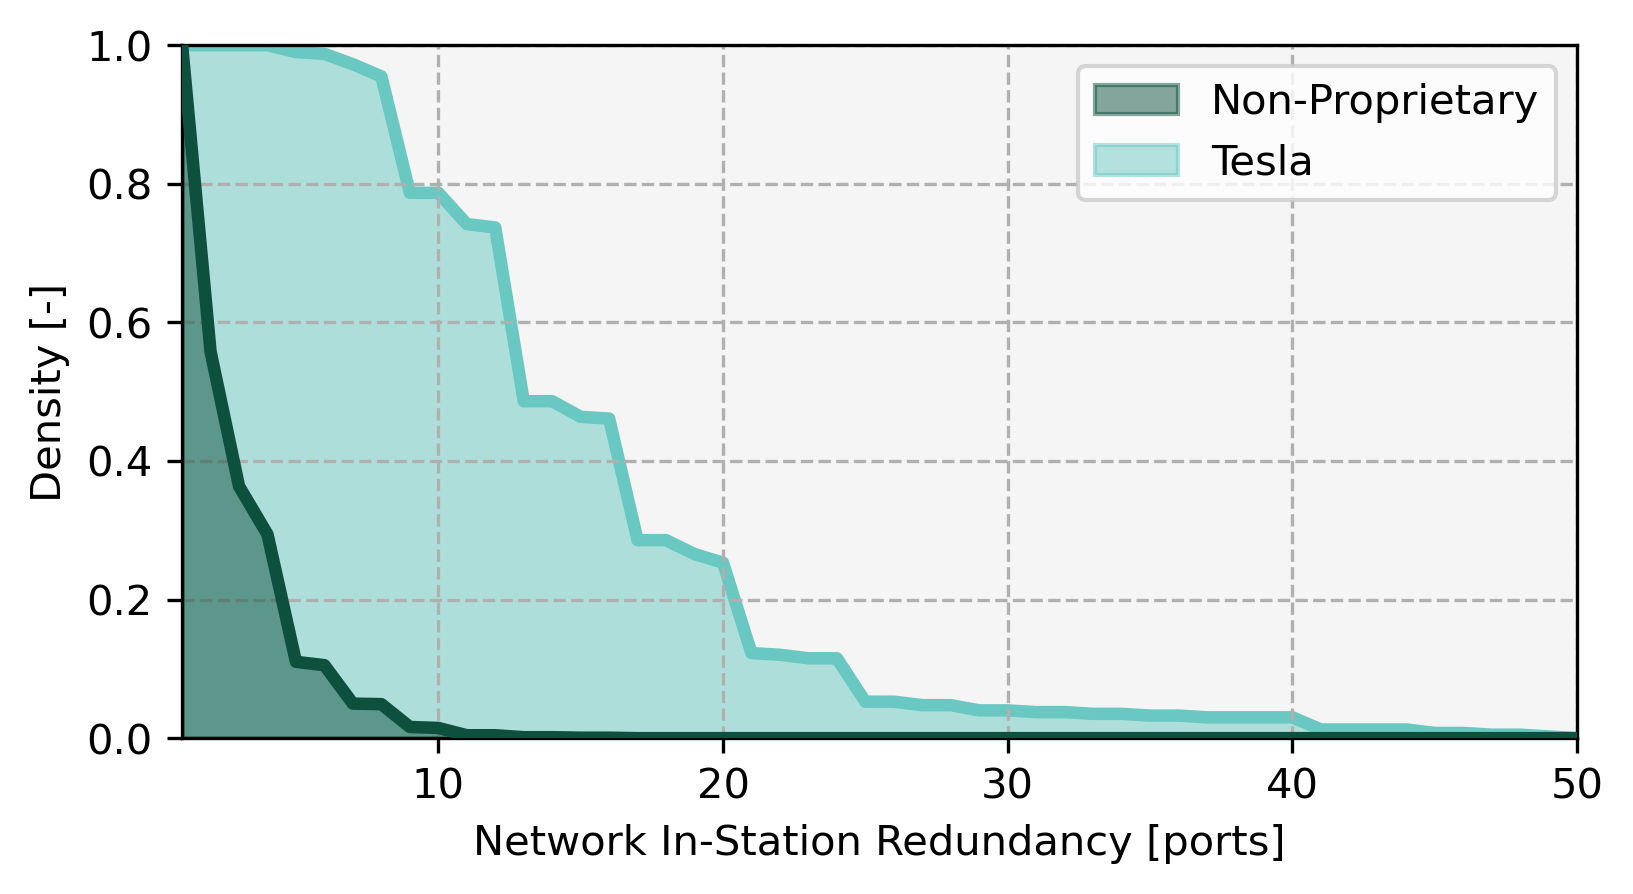
\includegraphics[width = \linewidth]{figs/California_RIS_Hist.png}
	\end{subfigure}
	\begin{subfigure}{\linewidth}
		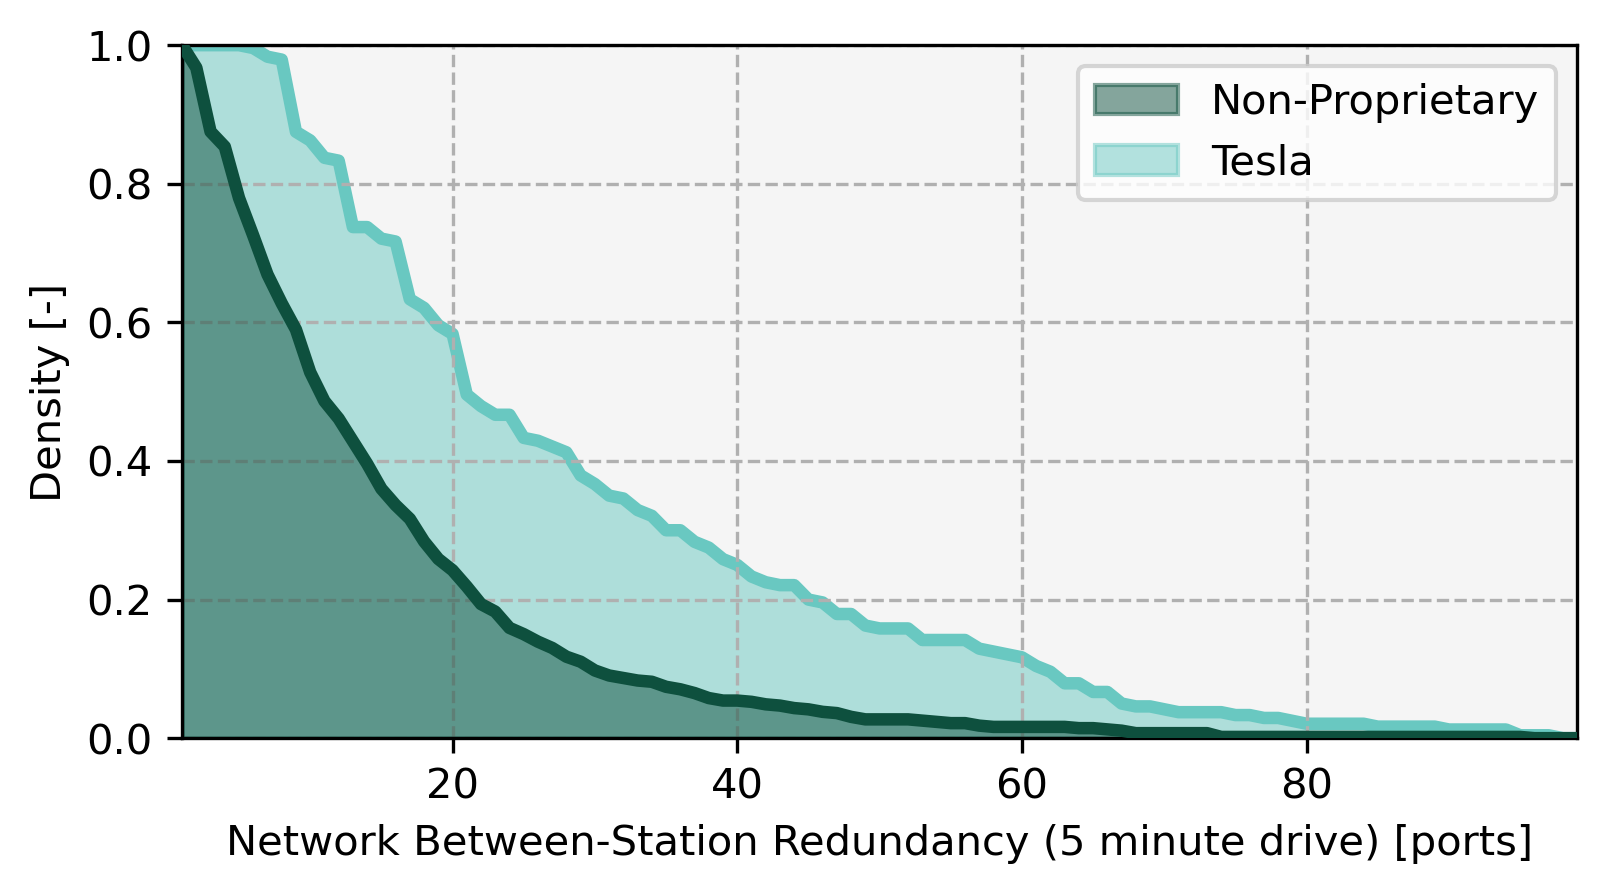
\includegraphics[width = \linewidth]{figs/California_RBS_Hist_300.png}
	\end{subfigure}
	\begin{subfigure}{\linewidth}
		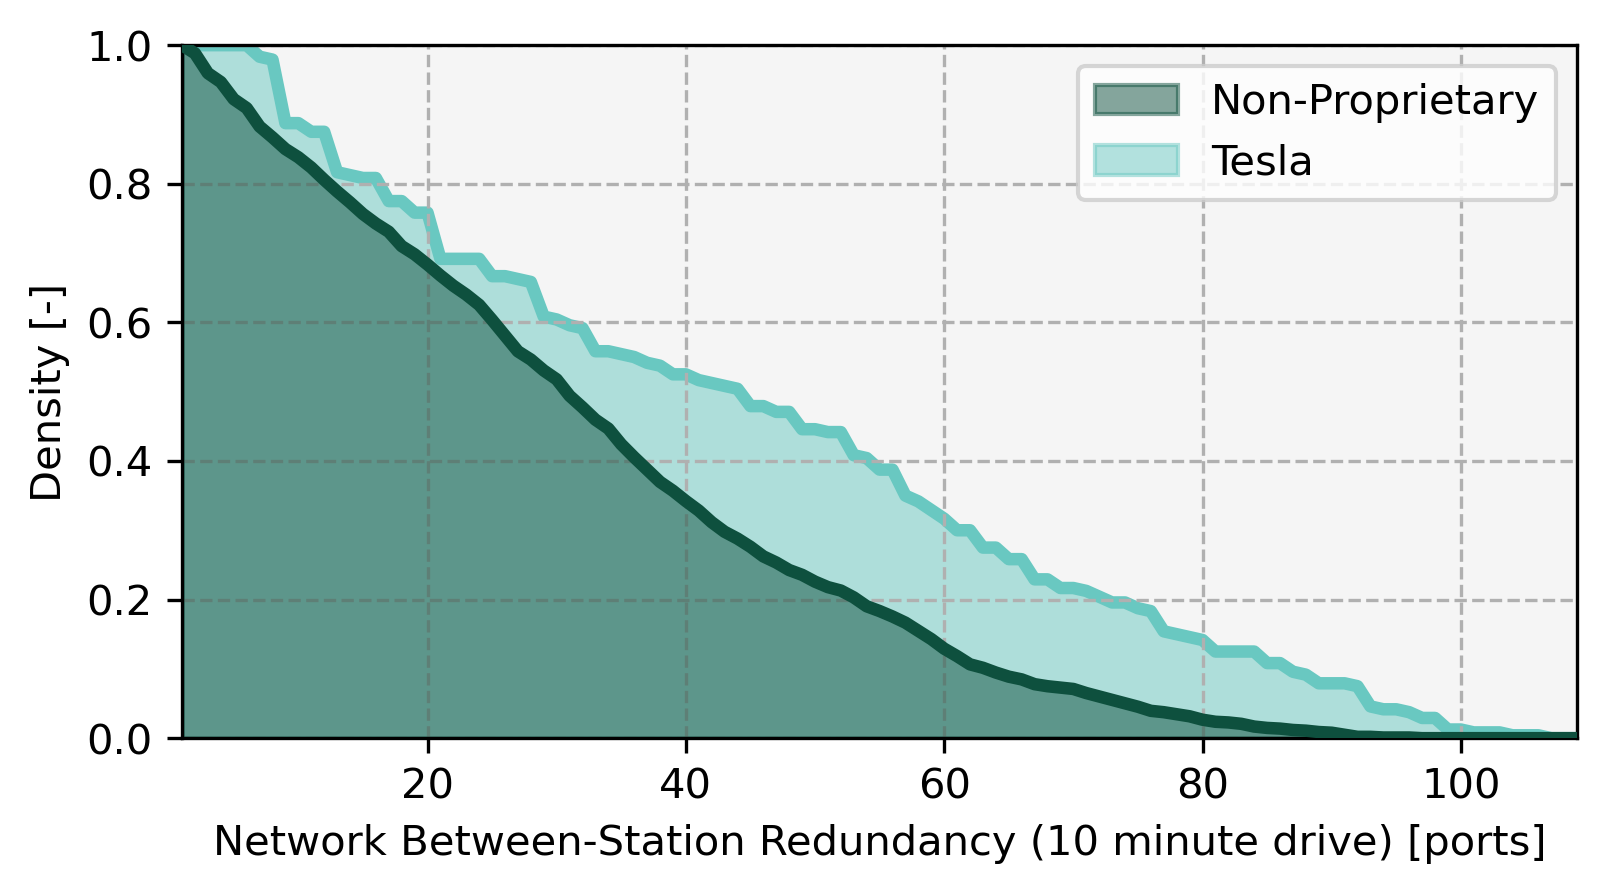
\includegraphics[width = \linewidth]{figs/California_RBS_Hist_600.png}
	\end{subfigure}
	%	\begin{subfigure}{\linewidth}
		%		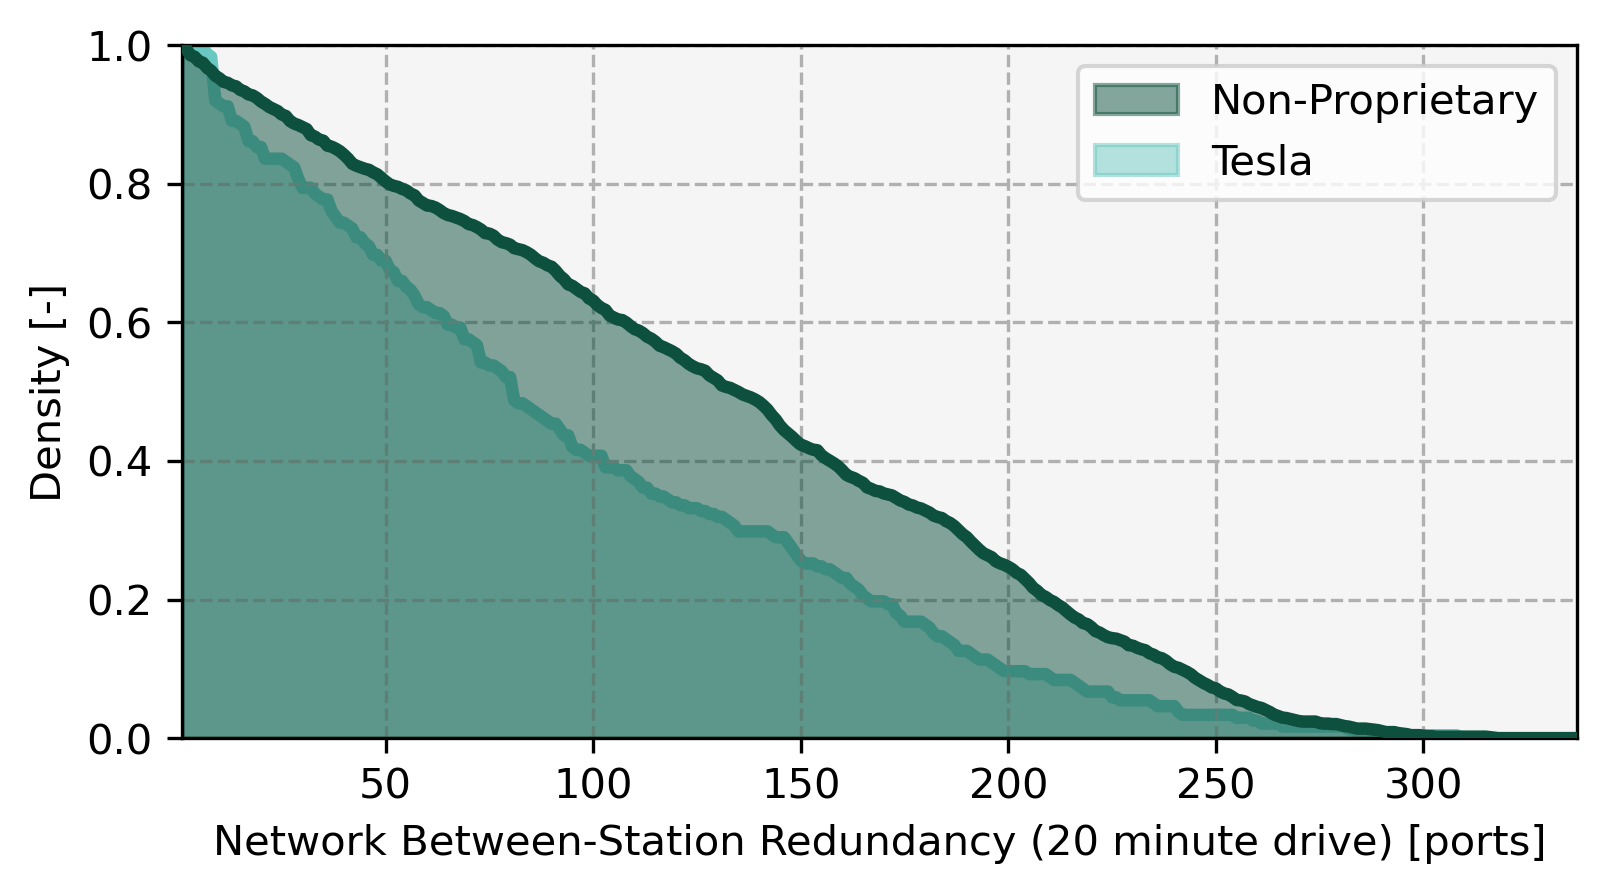
\includegraphics[width = \linewidth]{figs/California_RBS_Hist_1200.png}
		%	\end{subfigure}
	\caption{Survival functions for charger networks in California. Top panel shows survival function for in-station redundancy. Bottom three panels show survival functions for between-station redundancy for station cliques defined by 5 and 10 minute drive-times respectively.}
	\label{fig:network_histograms}
\end{figure}


\subsection*{Example}

Consider, as an example, the following four scenarios for a driver based out of Fresno:


\begin{compactenum}
	\item Risk neutral driver using a generic \gls{icev} with an \gls{ess} capacity of 550 kWh and an efficiency of 2700 kJ/km.
	\item Risk neutral driver using a Tesla Model 3 with an 80 kWh battery and efficiency of 536.4 kJ/km capable of charging at a max rate of 170 kW. The driver uses the Tesla DC station network exclusively and this network has high charger up-time (97\%). The driver only charges to 80\% \gls{soc} for DC events.
	\item Risk-cautious driver using a Chevrolet Bolt EV with an 65 kWh battery and efficiency of 626.5 kJ/km capable of charging at a max rate of 55 kW. The driver uses various non-proprietary networks and these networks have low charger up-time (75\%). The driver only charges to 80\% \gls{soc} for DC events.
	\item Risk-aggressive driver using a Chevrolet Bolt EV with an 65 kWh battery and efficiency of 626.5 kJ/km capable of charging at a max rate of 55 kW. The driver uses various non-proprietary networks and these networks have low charger up-time (75\%). The driver only charges to 80\% \gls{soc} for DC events.
\end{compactenum}

Each of these drivers will have a different experience of California's road transportation system for long trips. The neutral-expectations of time to reach each of the selected locations in the case study are provided in Table \ref{tab:scenarios} (driver is required to arrive at each destination with  at least 20\% \gls{soc}).

\begin{table}[H]
	\centering
	\caption{Neutral expectation of hours to locations from Fresno for example scenarios.}
	\label{tab:scenarios}
	\begin{tabular}{|C{.17\linewidth}|C{\linewidth * 1 / 5}|C{\linewidth * 1 / 5}|C{\linewidth * 1 / 5}|C{.23\linewidth}|}
		\hline Index & \gls{icev} & Model 3 Neutral & Bolt Cautious & Bolt Aggressive \\
		\hline 0 & 8.79 & 9.28 & 15.58 & 13.66 \\
		\hline 1 & 6.73 & 7.07 & 13.31 & 10.04 \\
		\hline 2 & 5.28 & 5.60 & 8.78 & 8.35 \\
		\hline 3 & 4.40 & 4.54 & 7.54 & 5.96 \\
		\hline 4 & 4.63 & 4.74 & 7.85 & 6.34 \\
		\hline 5 & 2.79 & 2.82 & 4.01 & 4.17 \\
		\hline 6 & 2.09 & 2.09 & 2.09 & 2.09 \\
		\hline 7 & 3.08 & 3.18 & 4.34 & 4.50 \\
		\hline 8 & 2.71 & 2.71 & 2.71 & 2.71 \\
		\hline 9 & 0.00 & 0.00 & 0.00 & 0.00 \\
		\hline 10 & 5.86 & 6.13 & 8.88 & 9.05 \\
		\hline 11 & 1.64 & 1.64 & 1.64 & 1.64 \\
		\hline 12 & 3.32 & 3.32 & 4.72 & 4.73 \\
		\hline 13 & 6.80 & 7.31 & 11.21 & 10.50 \\
		\hline 14 & 5.29 & 5.47 & 8.41 & 8.32 \\
		\hline
	\end{tabular}
\end{table}

The example drivers have very different experiences and perceived experiences. While the \gls{icev} driver can take the "direct" path (not deviating to find a station), the \gls{bev} drivers have to deviate from the "direct" path and require substantial time to charge. However, there is quite significant disparity within the set of proposed \gls{bev} drivers. For destinations which are within full-charge range, there is no difference between any of the drivers experiences. However, due to the lower range, lower max charge rate, and lower infrastructure reliability for the Bolt, the differentials between it and the Model 3 can be tremendous, especially for proximate and remote locations. It is worth noting, also, that the \gls{icev} and Model 3 are often able to take more direct routes. Table \ref{tab:scenarios_nc} shows the optimal route times with charging/fueling times removed.

\begin{table}[H]
	\centering
	\caption{Neutral expectation of hours to locations from Fresno for example scenarios without charging/fueling time.}
	\label{tab:scenarios_nc}
	\begin{tabular}{|C{.17\linewidth}|C{\linewidth * 1 / 5}|C{\linewidth * 1 / 5}|C{\linewidth * 1 / 5}|C{.23\linewidth}|}
		\hline Index & \gls{icev} & Model 3 Neutral & Bolt Cautious & Bolt Aggressive \\
		\hline 0 & 8.76 & 8.80 & 9.58 & 8.76 \\
		\hline 1 & 6.71 & 6.75 & 7.31 & 6.72 \\
		\hline 2 & 5.26 & 5.34 & 5.78 & 5.33 \\
		\hline 3 & 4.39 & 4.42 & 4.54 & 4.39 \\
		\hline 4 & 4.63 & 4.63 & 4.85 & 4.67 \\
		\hline 5 & 2.78 & 2.82 & 2.81 & 2.81 \\
		\hline 6 & 2.09 & 2.09 & 2.09 & 2.09 \\
		\hline 7 & 3.07 & 3.07 & 3.07 & 3.07 \\
		\hline 8 & 2.71 & 2.71 & 2.71 & 2.71 \\
		\hline 9 & 0.00 & 0.00 & 0.00 & 0.00 \\
		\hline 10 & 5.86 & 5.89 & 5.88 & 5.86 \\
		\hline 11 & 1.64 & 1.64 & 1.64 & 1.64 \\
		\hline 12 & 3.32 & 3.32 & 3.32 & 3.32 \\
		\hline 13 & 6.79 & 6.93 & 6.81 & 7.14 \\
		\hline 14 & 5.28 & 5.28 & 5.41 & 5.28 \\
		\hline
	\end{tabular}
\end{table}

The differences in total expected travel time between the \gls{icev} and Model 3 are relatively small and in the range of 5-10\% of travel time, a testament to Tesla's DC station network. Some would argue that this difference is unimportant as Tesla drivers can charge their vehicles while stopping for meals or during other natural breaks. This logic has been used to show that \glspl{bev} may approach convenience parity with \glspl{icev} in good circumstances \cite{Dixon_2020}. However, where such breaks are optional for \gls{icev} drivers, they are mandatory for \gls{bev} drivers and must be taken at specific points throughout the trip to coincide with charging. The loss of optionality must be accounted an inconvenience even if breaks would be taken in any event.

\subsection*{Experiment}

In order to gain an understanding of the effects of vehicular, infrastructural, and individual characteristics on transportation accessibility for long trips in California a designed experiment was conducted on the parameters in Table \ref{tab:exp_parameters}.

\begin{table}[H]
	\centering
	\caption{Parameters and levels for designed experiment}
	\label{tab:exp_parameters}
	\begin{tabular}{|C{.5\linewidth}|C{.5\linewidth}|}
		\hline Parameter & Levels \\
		\hline Charger Network & [Tesla, Non-Proprietary] \\
		\hline Range/Max Charge Multiplier & [1, 1.25, 1.5] \\
		\hline Charger Reliability & [.75, .85, .95] \\
		\hline Risk Attitude & [Cautious, Neutral, Aggressive] \\
		\hline
	\end{tabular}
\end{table}

The parameters and levels selected reflect possible ways to mitigate the disparity between \glspl{bev} and \glspl{icev} and within both sets. The rationale behind the selection of levels is as follows. As mentioned previously, the Tesla and non-proprietary DC charging networks are, presently, effectively separate and unequal entities. The base vehicle models in this study are the Chevrolet Bolt and Tesla Model 3 both of which are low-end vehicles for their category with more expensive models coming with higher battery capacities and charge rates \cite{AFDC_EVs_2023}. The range of reliability rates was taken from references \cite{Rempel_2023} with an aspirational high reliability rate added. Finally, risk attitudes were modeled on the theoretical basis outlined in the Methods section using \eqref{eq:superquantile} with Cautious ($p_0 = .5,\ p_1 = 1$), Neutral ($p_0 = 0,\ p_1 = 1$), and Aggressive ($p_0 = 0,\ p_1 = .5$) drivers.

The metric used for comparison is long-trip accessibility as defined in \eqref{eq:a} where the cost used is total route time. In each case the optimal-path tree $P$ is computed using a stochastic, constrained implementation of Dijkstra's method as described in the Methods section with sample vectors of length 100. On average the difference between the accessibility score $A$ for the Model 3 and Bolt was 2.72 hours in favor of the Model 3 for the same combinations of experimental parameters. This difference is due to the superior range, charging rate, and DC charging infrastructure enjoyed by the Model 3. Linear regression was performed on the experimental parameters, interactions and results. Significant parameters ($\alpha = 0.05$) for the Bolt and Model 3 are listed in Tables \ref{tab:sp_bolt} and \ref{tab:sp_model_3} respectively.

\begin{table}[H]
	\centering
	\caption{Significant ($\alpha = 0.05$) terms from linear regression for Bolt.}
	\label{tab:sp_bolt}
	\begin{tabular}{|C{.6\linewidth}|C{.2\linewidth}|C{.2\linewidth}|}
		\hline Parameter & $\beta$ & p-value \\
		\hline {\small Intercept } & 8.557 & 0.000 \\
		\hline {\small Multiplier } & -2.127 & 0.000 \\
		\hline {\small Attitude[T.Neutral] } & 0.775 & 0.004 \\
		\hline {\small Attitude[T.Cautious] } & 1.188 & 0.000 \\
		\hline
	\end{tabular}
\end{table}

\begin{table}[H]
	\centering
	\caption{Significant ($\alpha = 0.05$) terms from linear regression for Model 3.}
	\label{tab:sp_model_3}
	\begin{tabular}{|C{.6\linewidth}|C{.2\linewidth}|C{.2\linewidth}|}
		\hline Parameter & $\beta$ & p-value \\
		\hline {\small Intercept } & 5.840 & 0.000 \\
		\hline {\small Multiplier } & -0.118 & 0.000 \\
		\hline
	\end{tabular}
\end{table}


\begin{table}[H]
	\centering
	%	\caption{Significant ($\alpha = 0.05$) terms from linear regression for Bolt.}
	%	\label{tab:sp_bolt}
	\begin{tabular}{|C{.6\linewidth}|C{.2\linewidth}|C{.2\linewidth}|}
		\hline Parameter & $\beta$ & p-value \\
		\hline {\small Intercept } & 6.678 & 0.000 \\
		\hline {\small Range } & -0.903 & 0.035 \\
		\hline {\small Attitude } & 2.633 & 0.000 \\
		\hline {\small Attitude:Range } & -2.570 & 0.000 \\
		\hline {\small Attitude:Reliability } & -2.028 & 0.003 \\
		\hline {\small Attitude:Non-Tesla Access } & 1.406 & 0.021 \\
		\hline
	\end{tabular}
\end{table}

\begin{table}[H]
	\centering
	%	\caption{Significant ($\alpha = 0.05$) terms from linear regression for Bolt.}
	%	\label{tab:sp_bolt}
	\begin{tabular}{|C{.6\linewidth}|C{.2\linewidth}|C{.2\linewidth}|}
		\hline Parameter & $\beta$ & p-value \\
		\hline {\small Intercept } & 6.800 & 0.000 \\
		\hline {\small Range } & -0.921 & 0.012 \\
		\hline {\small Attitude } & 3.640 & 0.000 \\
		\hline {\small Attitude:Range } & -3.559 & 0.000 \\
		\hline {\small Attitude:Reliability } & -2.772 & 0.000 \\
		\hline {\small Attitude:Redundancy-IS } & -1.339 & 0.026 \\
		\hline {\small Attitude:Range:Reliability } & 2.754 & 0.002 \\
		\hline
	\end{tabular}
\end{table}

The regression results support the intuitive conclusion that vehicle range is important in determining long-trip accessibility. A longer range vehicle will have more long-trip accessibility for a region of a given size. It is somewhat surprising that charger reliability was not significant for either vehicle/supply network combination. The lack of significance of reliability in the experimental range is due to the redundancy present in both supply networks. Where the Tesla DC charger network consists of stations with many chargers the non-proprietary network consists of smaller stations in closer proximity to one-another. Because there are more chargers total in the Tesla network and because these are redundant within stations rather than between stations the effect of non-functional chargers on user experience is lesser. A consequence of the more distributed non-proprietary network is that charger non-availability can catch a driver out and require a costly event relocation or even a tow. For this reason, driver risk attitude is more important for non-Tesla drivers for whom the trade-off between more direct routes with higher risk and less direct routes with lower risk is substantial. Overall the results indicate that the reliability of individual chargers is less important than their distribution and that the non-proprietary DC charging network is currently inferior to the Tesla DC charging network in California.

In the past, and still largely in the present, the Tesla DC charging network has been sequestered for the use of Tesla drivers. Recently, with the introduction of the NACS standard, this restriction has started to loosen. In the future, the Tesla and non-Tesla networks will function, increasingly, as one. A comparison of accessibility for each vehicle with each network independently, and the combined network is shown in Table \ref{tab:vehicles_networks}.

\begin{table}[H]
	\centering
	\caption{Accessibility for Bolt and Model 3 with neutral driver for various networks.}
	\label{tab:vehicles_networks}
	\begin{tabular}{|C{.4\linewidth}|C{.3\linewidth}|C{.3\linewidth}|}
		\hline Network & Bolt & Model 3 \\
		\hline Non-Proprietary & 9.49 & 6.32 \\
		\hline Tesla & 7.63 & 5.85 \\
		\hline Combined & 7.63 & 5.85 \\
		\hline
	\end{tabular}
\end{table}

The results show that the experience of Bolt drivers is improved by being able to use the Tesla DC charging network but does not redress the gap to Teslas using the Tesla network. Tesla drivers experiences are worsened by being only able to use the non-proprietary network but not to the same extent as those of Bolt drivers. It is notable that for the combined network both vehicles made exclusive use of Tesla DC charging stations. Given the demonstrated superiority of the Tesla network one might suppose that its opening will markedly improve the experience of non-Tesla drivers while failing to improve that of Tesla drivers. In fact, it may deteriorate Tesla driver experience due to higher demand at Tesla DC charging stations.

That the Tesla network is preferable to the non-proprietary network is due to redundancy. The Tesla network in California has roughly twice the number of chargers as the non-proprietary network with less than 30\% of the stations. Redundancy is not trivial to quantify for a network. Tesla chargers reinforce Tesla chargers within station but the distances between stations are large. Non-proprietary chargers reinforce between stations with smaller distances between. There is reason to suspect that even if the number of non-proprietary chargers were doubled but the distribution remained similar that Tesla's network would be preferable. The difference is informational. Where a driver finds a queue at a small station, that driver has uncertain information about the availability of chargers at proximate stations. Further, should that driver relocate to another station and find a similar or larger queue there is no mechanism to return to the vacated queue position at the previous station. This issue is more relevant for long-trips tahn it is for routine charging as the former generates less flexible charging demand. Policy makers should carefully consider which type of redundancy their policies encourage and what effects this will have. Quantifying the impacts of this informational issue is out of scope for this study and will be the subject of future research.

\section*{Conclusions}

Transportation accessibility is a very useful framework for policymakers and planners as it allows for the simultaneous consideration of land-use and transportation. For long trips, the land use component becomes exogenous in the short and medium term and the differentiating factor is transportation. Consideration of long road trips plays a role in vehicle selection out of proportion with their regularity encouraging continued \gls{icev} retention at the individual and household level. Quantifying the disadvantages of \glspl{bev} compared to \glspl{icev} is critical in addressing this issue. The framework and methodology developed are a valuable tool for th origination and evaluation of future policy.

In this study a framework for accessing long-trip accessibility for road vehicles in a region is developed. Using this framework and current data, a case study for the state of California was conducted comparing long-trip accessibility between \glspl{icev} and \glspl{bev} and between different \glspl{bev}. Results show that \glspl{icev} retain an advantage over \glspl{bev} of all types but this advantage is marginal for Tesla vehicles but major for low-end non-Tesla vehicles. the major difference is access to the Tesla DC charging network which is larger and differently structured compared to the non-proprietary networks. Specifically, the Tesla DC fast charging network is concentrated in large stations providing redundancy within station where the non-proprietary networks consist of distributed small stations providing redundancy between stations. The different approaches between Tesla and non-proprietary networks are due to the economic circumstances under which they developed. Policymakers and planners should note the differences between them and the effects these have on long-trip accessibility in considering new incentive programs.